\item \textbf{{[}RVHS/PRELIM/9597/2019/P1/Q4{]} }

\textbf{Begemed }

Begemed is a casual game which is played on ruled grids. The player
is required to swap a gem in one of the four possible directions,
namely \textquotedblleft up\textquotedblright , \textquotedblleft down\textquotedblright ,
\textquotedblleft left\textquotedblright , \textquotedblleft right\textquotedblright ;
after the swap, if a row or a column of 3 or more gems are formed,
it\textquoteright s considered a valid move and the connected gems
will be destroyed. Otherwise, it\textquoteright s considered an invalid
move. Note that diagonal directions are not counted. 

Below are some examples of the game demonstrated in a $5\times5$
grid. The letters \textquotedbl d\textquotedbl , \textquotedbl s\textquotedbl ,
\textquotedbl t\textquotedbl , \textquotedbl r\textquotedbl ,
\textquotedbl e\textquotedbl{} represents Diamond, Sapphire, Topaz,
Ruby, Emerald respectively. 
\begin{center}
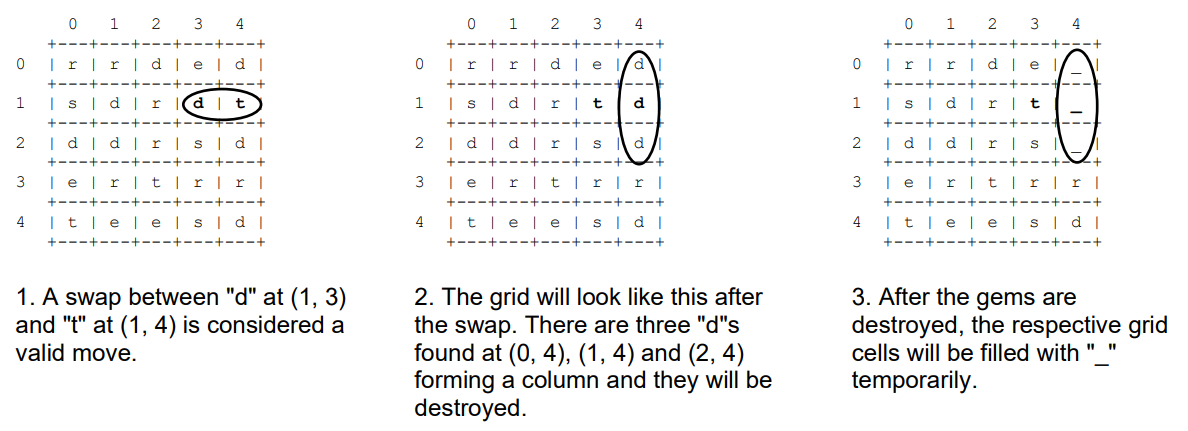
\includegraphics[width=0.7\paperwidth]{C:/Users/Admin/Desktop/Github/question_bank/LyX/static/img/9597-RVHS-2019-P1-Q4-1}
\par\end{center}

Some other valid swaps are: 
\begin{center}
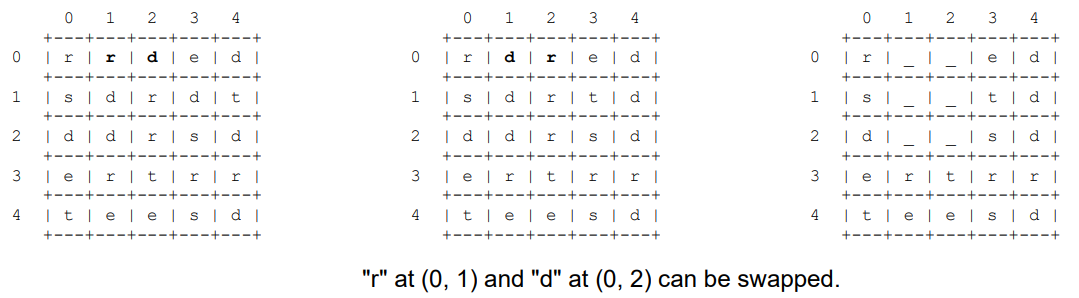
\includegraphics[width=0.7\paperwidth]{C:/Users/Admin/Desktop/Github/question_bank/LyX/static/img/9597-RVHS-2019-P1-Q4-2}
\par\end{center}

\begin{center}
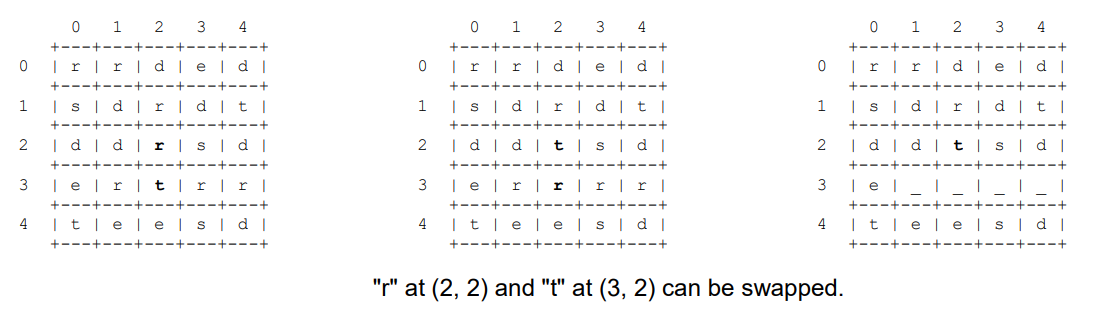
\includegraphics[width=0.7\paperwidth]{C:/Users/Admin/Desktop/Github/question_bank/LyX/static/img/9597-RVHS-2019-P1-Q4-3}
\par\end{center}

\begin{center}
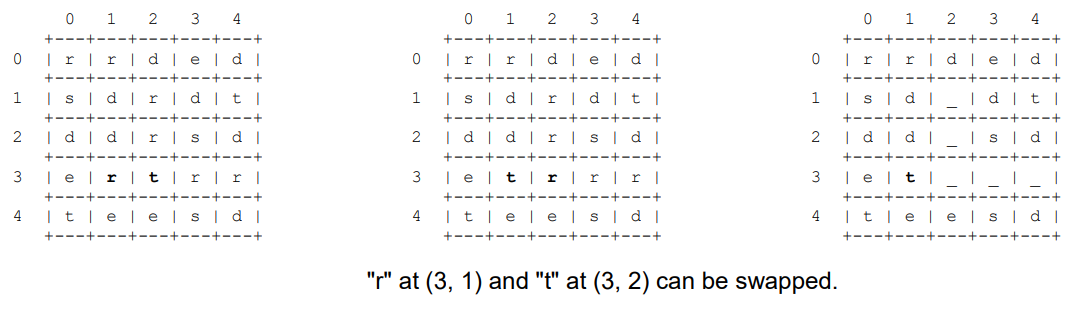
\includegraphics[width=0.7\paperwidth]{C:/Users/Admin/Desktop/Github/question_bank/LyX/static/img/9597-RVHS-2019-P1-Q4-4}
\par\end{center}

You are tasked to create a text-based interactive \textquotedblleft Begemed\textquotedblright{}
game in the following tasks. 

\subsection*{Task 4.1 }

Implement \texttt{Begemed} class according to the UML class diagram
and attributes/methods specifications given. 
\begin{center}
\begin{tabular}{|l|}
\hline 
\texttt{Board}\tabularnewline
\hline 
\texttt{- board: list }\tabularnewline
\hline 
\texttt{+ Board(size: int)}\tabularnewline
\texttt{+ new\_game(board: list) }\tabularnewline
\texttt{+ check\_connection(row: int, col: int): boolean }\tabularnewline
\texttt{+ find\_valid\_moves(row: int, col: int): list}\tabularnewline
\texttt{+ display(hint: boolean=False)}\tabularnewline
\hline 
\end{tabular}
\par\end{center}

\begin{center}
\begin{tabular}{|l|l|}
\hline 
\texttt{\textbf{Attribute}} & \texttt{\textbf{Specification}}\tabularnewline
\hline 
\texttt{board: list} & \texttt{board} is a 2-dimensional \texttt{list} hosting the gems inside
each grid. \tabularnewline
\hline 
\end{tabular}
\par\end{center}

Methods and its specification.
\begin{itemize}
\item \texttt{Board(n: int) : n} is the size used to define the dimension
of the \texttt{board}. The board should be initialized to a ($n\times n$)
2- dimensional list filled with string \textquotedblleft \_\textquotedblright .
\hfill{}{[}2{]}
\item \texttt{new\_game(new\_board : list): new\_game} takes in a \texttt{list}
named \texttt{new\_board} and assign it to the class attribute \texttt{board}.
The following list is provided in the python template file. 

t\texttt{est\_board = {[} {[}'r', 'r', 'd', 'e', 'd'{]}, {[}'s', 'd',
'r', 'd', 't'{]}, {[}'d', 'd', 'r', 's', 'd'{]}, {[}'e', 'r', 't',
'r', 'r'{]}, {[}'t', 'e', 'e', 's', 'd'{]}{]} }

\emph{This method is just a temporary solution which help you in initial
coding and debugging. In a later task, there will be further instructions
to update its implementation.} \hfill{}{[}1{]}
\item \texttt{check\_connection( row: int, col: int): boolean : check\_connection}
takes in the \texttt{row} and \texttt{col} value of a particular gem,
then check if there is a connection of 3 or more gems of the same
type in its horizontal or vertical direction. Return \texttt{True}
if such a connection is found, and \texttt{False} otherwise. \hfill{}{[}8{]}
\end{itemize}

\subsection*{Evidence 24 }

Program code of class Board and class methods up to \texttt{check\_conection}.
{[}11{]} 

Methods and its specification.
\begin{itemize}
\item \texttt{find\_valid\_moves( row: int, col: int): list} : \texttt{find\_valid\_moves}
takes in the \texttt{row} and \texttt{col} value of a particular gem,
then attempt to swap in the four directions (up, down, left, right).
If there is a new connection of 3 or more gems of the same type formed,
record as a valid movement. 

Return a \texttt{list} containing all valid movements. An empty \texttt{list}
is to be returned if no valid movement is found. 

For example:

\noindent %
\noindent\begin{minipage}[t]{1\columnwidth}%
\texttt{~~~~0~~~1~~~2~~~3~~~4 }

\texttt{~~+-{}-{}-+-{}-{}-+-{}-{}-+-{}-{}-+-{}-{}-+ }

\texttt{0 | r | r | d | e | d | }

\texttt{~~+-{}-{}-+-{}-{}-+-{}-{}-+-{}-{}-+-{}-{}-+ }

\texttt{1 | s | d | r | d | t | }

\texttt{~~+-{}-{}-+-{}-{}-+-{}-{}-+-{}-{}-+-{}-{}-+ }

\texttt{2 | d | d | r | s | d | }

\texttt{~~+-{}-{}-+-{}-{}-+-{}-{}-+-{}-{}-+-{}-{}-+ }

\texttt{3 | e | r | t | r | r | }

\texttt{~~+-{}-{}-+-{}-{}-+-{}-{}-+-{}-{}-+-{}-{}-+ }

\texttt{4 | t | e | e | s | d | }

\texttt{~~+-{}-{}-+-{}-{}-+-{}-{}-+-{}-{}-+-{}-{}-+ }%
\end{minipage}

If \texttt{find\_valid\_moves(0, 2)} is called, the function should
return \texttt{{[}'d', 'l'{]}} because when down swap or left swap
is performed on gem at \texttt{(0, 2)}, a new connection of 3 or more
gems of the same type will be formed. {[}5{]}
\item \texttt{display(hint: Boolean=False)} : \texttt{display} will print
out the \texttt{board} according to the sample format given. Take
note that the \texttt{size} of the board can be changed and hence
the grid outline should be dynamically adjusted according to its \texttt{size}. 

For example: 

\noindent %
\noindent\begin{minipage}[t]{1\columnwidth}%
\texttt{~~~~0~~~1~~~2~~~3~~~4}

\texttt{~~+-{}-{}-+-{}-{}-+-{}-{}-+-{}-{}-+-{}-{}-+}

\texttt{0 | r | r | d | e | d |}

\texttt{~~+-{}-{}-+-{}-{}-+-{}-{}-+-{}-{}-+-{}-{}-+}

\texttt{1 | s | d | r | d | t |}

\texttt{~~+-{}-{}-+-{}-{}-+-{}-{}-+-{}-{}-+-{}-{}-+}

\texttt{2 | d | d | r | s | d |}

\texttt{~~+-{}-{}-+-{}-{}-+-{}-{}-+-{}-{}-+-{}-{}-+}

\texttt{3 | e | r | t | r | r |}

\texttt{~~+-{}-{}-+-{}-{}-+-{}-{}-+-{}-{}-+-{}-{}-+}

\texttt{4 | t | e | e | s | d |}

\texttt{~~+-{}-{}-+-{}-{}-+-{}-{}-+-{}-{}-+-{}-{}-+}%
\end{minipage}

\texttt{hint} is an optional argument with a default value of \texttt{False}.
If \texttt{hint} is set to be \texttt{True}, the gems with valid moves
should be highlighted by using the \textbf{uppercase} letters, and
the valid moves for the \textbf{coordinates} and \textbf{directions}
should be displayed too. 

For example: 

\noindent %
\noindent\begin{minipage}[t]{1\columnwidth}%
\texttt{(0, 1) {[}'r'{]}}

\texttt{(0, 2) {[}'d', 'l'{]}}

\texttt{(1, 2) {[}'u'{]} }

\texttt{(1, 3) {[}'u', 'r'{]}}

\texttt{(2, 2) {[}'d'{]} }

\texttt{(3, 0) {[}'d'{]} }

\texttt{(3, 1) {[}'r'{]}}

\texttt{(3, 3) {[}'l'{]} }%
\end{minipage}

\noindent %
\noindent\begin{minipage}[t]{1\columnwidth}%
\texttt{~~~~0~~~1~~~2~~~3~~~4}

\texttt{~~+-{}-{}-+-{}-{}-+-{}-{}-+-{}-{}-+-{}-{}-+}

\texttt{0 | r | }\texttt{\textbf{\uline{R}}}\texttt{ | }\texttt{\textbf{\uline{D}}}\texttt{
| e | d |}

\texttt{~~+-{}-{}-+-{}-{}-+-{}-{}-+-{}-{}-+-{}-{}-+}

\texttt{1 | s | d | }\texttt{\textbf{\uline{R}}}\texttt{ | }\texttt{\textbf{\uline{D}}}\texttt{
| t |}

\texttt{~~+-{}-{}-+-{}-{}-+-{}-{}-+-{}-{}-+-{}-{}-+}

\texttt{2 | d | d | }\texttt{\textbf{\uline{R}}}\texttt{ | s |
d |}

\texttt{~~+-{}-{}-+-{}-{}-+-{}-{}-+-{}-{}-+-{}-{}-+}

\texttt{3 | }\texttt{\textbf{\uline{E}}}\texttt{ | }\texttt{\textbf{\uline{R}}}\texttt{
| t | }\texttt{\textbf{\uline{R}}}\texttt{ | r |}

\texttt{~~+-{}-{}-+-{}-{}-+-{}-{}-+-{}-{}-+-{}-{}-+}

\texttt{4 | t | e | e | s | d |}

\texttt{~~+-{}-{}-+-{}-{}-+-{}-{}-+-{}-{}-+-{}-{}-+}%
\end{minipage}
\end{itemize}

\subsection*{Evidence 25 }

Program code of class method \texttt{find\_valid\_moves} and \texttt{display}.
\hfill{}{[}14{]}

\subsection*{Task 4.2 }

Write a texted based menu which has the following options. Validation
of the user input is needed. 

\noindent %
\noindent\begin{minipage}[t]{1\columnwidth}%
\texttt{Choose an option below: }

\texttt{1) Validate Move }

\texttt{2) Toggle Hint Mode}

\texttt{3) Move the Gem!}

\texttt{4) New Game}

\texttt{5) Exit }%
\end{minipage}

The descriptions for the options can be found below. 

Options and its descriptions.
\begin{itemize}
\item \texttt{Validate Move} : Ask user to input a set of \texttt{row},
\texttt{col} and \texttt{direction}. Check and feedback if this swap
is valid. 
\item \texttt{Toggle Hint Mode} : For every new game, the \texttt{hint}
mode by default should be \texttt{off}. Use this option to toggle
the \texttt{on} and \texttt{off} state of hint mode.

If \texttt{hint} mode is \texttt{on}, the menu interface should automatically
highlight the gems with valid moves and print out a list of the coordinates
together with its valid movement directions. 
\item \texttt{Move the Gem! :} Move a gem in a chosen direction. 

\emph{Note that the related class method will only be implemented
in the }\textbf{\emph{next task}}\emph{. For the current menu, you
only need to take in user input for }\texttt{row}\emph{, }\texttt{col}\emph{
and }\texttt{direction}\emph{, but no further action needs to be taken. }
\item \texttt{New Game} : Start a new game and reset \texttt{hint} mode
to be off. 

For this task, you may just initialize the new game using the \texttt{test\_board}
given. 
\item \texttt{Exit} : Exit program. 
\end{itemize}

\subsection*{Evidence 26}

Program code of menu implementation. \hfill{}{[}10{]}

\subsection*{Task 4.3}

Update the class Begemed with the following methods. Note that this
task is time consuming and only worth \textbf{2 marks}. 

Methods and its specification.
\begin{itemize}
\item \texttt{new\_game(n: int)} : \texttt{new\_game} will now take in a
size of \texttt{n} and randomly generate a \texttt{$\mathtt{n}\times\mathtt{n}$}
board of gems. The newly generated gems should not have any connection
of 3 or more gems with the same type. 
\item \texttt{move\_gem(row: int, col: int, direction: string)} \texttt{move\_gem}
should take in a gem position and direction. If the swap is a valid
move, detect any newly formed connection of 3 or more gems with the
same type and cancel them. 

\noindent %
\begin{minipage}[t]{0.5\columnwidth}%
\texttt{~~~~0~~~1~~~2~~~3~~~4 }

\texttt{~~+-{}-{}-+-{}-{}-+-{}-{}-+-{}-{}-+-{}-{}-+ }

\texttt{0 | r | r | d | e | d |}

\texttt{~~+-{}-{}-+-{}-{}-+-{}-{}-+-{}-{}-+-{}-{}-+ }

\texttt{1 | s | d | r | d | t |}

\texttt{~~+-{}-{}-+-{}-{}-+-{}-{}-+-{}-{}-+-{}-{}-+ }

\texttt{2 | d | d | r | s | d |}

\texttt{~~+-{}-{}-+-{}-{}-+-{}-{}-+-{}-{}-+-{}-{}-+ }

\texttt{3 | e | }\texttt{\textbf{\uline{r}}}\texttt{ | }\texttt{\textbf{\uline{t}}}\texttt{
| r | r |}

\texttt{~~+-{}-{}-+-{}-{}-+-{}-{}-+-{}-{}-+-{}-{}-+ }

\texttt{4 | t | e | e | s | d |}

\texttt{~~+-{}-{}-+-{}-{}-+-{}-{}-+-{}-{}-+-{}-{}-+}

Swap \textquotedbl r\textquotedbl{} at (3, 1) with \textquotedbl t\textquotedbl{}
at (3, 2)%
\end{minipage}%
\begin{minipage}[t]{0.5\columnwidth}%
\texttt{~~~~0~~~1~~~2~~~3~~~4 }

\texttt{~~+-{}-{}-+-{}-{}-+-{}-{}-+-{}-{}-+-{}-{}-+}

\texttt{0 | r | r | d | e | d | }

\texttt{~~+-{}-{}-+-{}-{}-+-{}-{}-+-{}-{}-+-{}-{}-+ }

\texttt{1 | s | d | \_ | d | t |}

\texttt{~~+-{}-{}-+-{}-{}-+-{}-{}-+-{}-{}-+-{}-{}-+ }

\texttt{2 | d | d | \_ | s | d | }

\texttt{~~+-{}-{}-+-{}-{}-+-{}-{}-+-{}-{}-+-{}-{}-+ }

\texttt{3 | e | t | \_ | \_ | \_ | }

\texttt{~~+-{}-{}-+-{}-{}-+-{}-{}-+-{}-{}-+-{}-{}-+ }

\texttt{4 | t | e | e | s | d | }

\texttt{~~+-{}-{}-+-{}-{}-+-{}-{}-+-{}-{}-+-{}-{}-+}

Gems connected with 3 or more of the same type are cancelled. %
\end{minipage}

After the gems are being cancelled, those gems on top of the current
gems should \textquotedblleft fall\textquotedblright{} down. 

New gems will be randomly generated to fill up the board. 

\noindent %
\begin{minipage}[t]{0.5\columnwidth}%
\texttt{~~~~0~~~1~~~2~~~3~~~4 }

\texttt{~~+-{}-{}-+-{}-{}-+-{}-{}-+-{}-{}-+-{}-{}-+ }

\texttt{0 | r | r | \_ | \_ | \_ | }

\texttt{~~+-{}-{}-+-{}-{}-+-{}-{}-+-{}-{}-+-{}-{}-+ }

\texttt{1 | s | d | \_ | }\texttt{\textbf{\uline{e}}}\texttt{ |
}\texttt{\textbf{\uline{d}}}\texttt{ |}

\texttt{~~+-{}-{}-+-{}-{}-+-{}-{}-+-{}-{}-+-{}-{}-+ }

\texttt{2 | d | d | \_ | }\texttt{\textbf{\uline{d}}}\texttt{ |
}\texttt{\textbf{\uline{t}}}\texttt{ |}

\texttt{~~+-{}-{}-+-{}-{}-+-{}-{}-+-{}-{}-+-{}-{}-+ }

\texttt{3 | e | t | }\texttt{\textbf{\uline{d}}}\texttt{ | }\texttt{\textbf{\uline{s}}}\texttt{
| }\texttt{\textbf{\uline{d}}}\texttt{ |}

\texttt{~~+-{}-{}-+-{}-{}-+-{}-{}-+-{}-{}-+-{}-{}-+ }

\texttt{4 | t | e | e | s | d | }

\texttt{~~+-{}-{}-+-{}-{}-+-{}-{}-+-{}-{}-+-{}-{}-+ }

Gems on top of the cancelled gem \textquotedblleft falls\textquotedblright{}
down%
\end{minipage}%
\begin{minipage}[t]{0.5\columnwidth}%
\texttt{~~~~0~~~1~~~2~~~3~~~4 }

\texttt{~~+-{}-{}-+-{}-{}-+-{}-{}-+-{}-{}-+-{}-{}-+ }

\texttt{0 | r | r | }\texttt{\textbf{\uline{r}}}\texttt{ | }\texttt{\textbf{\uline{s}}}\texttt{
| }\texttt{\textbf{\uline{s}}}\texttt{ |}

\texttt{~~+-{}-{}-+-{}-{}-+-{}-{}-+-{}-{}-+-{}-{}-+ }

\texttt{1 | s | d | }\texttt{\textbf{\uline{t}}}\texttt{ | e |
d | }

\texttt{~~+-{}-{}-+-{}-{}-+-{}-{}-+-{}-{}-+-{}-{}-+ }

\texttt{2 | d | d | }\texttt{\textbf{\uline{t}}}\texttt{ | d |
t | }

\texttt{~~+-{}-{}-+-{}-{}-+-{}-{}-+-{}-{}-+-{}-{}-+ }

\texttt{3 | e | t | d | s | d |}

\texttt{~~+-{}-{}-+-{}-{}-+-{}-{}-+-{}-{}-+-{}-{}-+ }

\texttt{4 | t | e | e | s | d |}

\texttt{~~+-{}-{}-+-{}-{}-+-{}-{}-+-{}-{}-+-{}-{}-+ }

New gems are generated %
\end{minipage}

Check if there are more connections of 3 or more gems of the same
type are formed, if found repeat the above cancel and refill steps. 
\item \texttt{menu} Adjust the menu to accommodate these new changes. 
\end{itemize}

\subsection*{Evidence 27 }

Program code of above mentioned changes. \hfill{}{[}2{]}